%%%%%%%%%%%%%%%%%%%%%%%%%%%%%%%%%%%%%%%%%%%%%%%%%%%%%%%%%%%%%%%%%%%%%%%%%%%%%
%	e-Yantra, IIT-Bombay

%	Document Author: Chinmay Patil
%	Date: 11-July,2016
%	Last Edited by: Chinmay
%   Date Last updated: 11-06-2016 

%%%%%%%%%%%%%%%%%%%%%%%%%%%%%%%%%%%%%%%%%%%%%%%%%%%%%%%%%%%%%%%%%%%%%%%%%%%%%


\documentclass[11pt,a4paper]{article}
\usepackage{graphicx}
\usepackage{listings}
\usepackage{graphics}
\usepackage{wrapfig}
\usepackage[T1]{fontenc}
\usepackage[margin=1.2in]{geometry}
\usepackage{tcolorbox}
\usepackage{hyperref}
\usepackage{dingbat}
\usepackage{float}
\usepackage{tocloft}

\begin{document}
\begin{titlepage}
\title{Sensor Data Format}
\author{e-Yantra Team}
\date{\today}
\maketitle
\end{titlepage}

\newpage
	\section{Sensor On Wiced Sense}
	
	
	\begin{figure}[h]
    \centering
	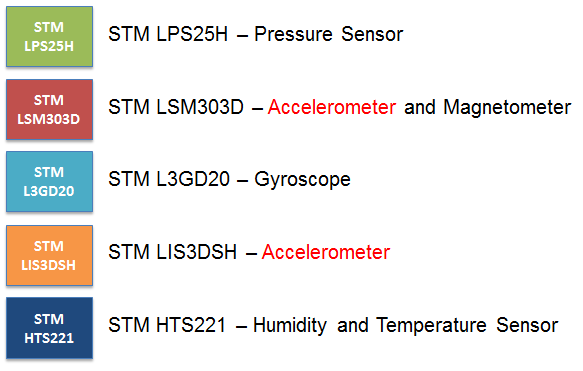
\includegraphics[scale=0.5]{Sensors.png}
	\end{figure}

\section{Sensor Packet Format}

\begin{figure}[h]
    \centering
	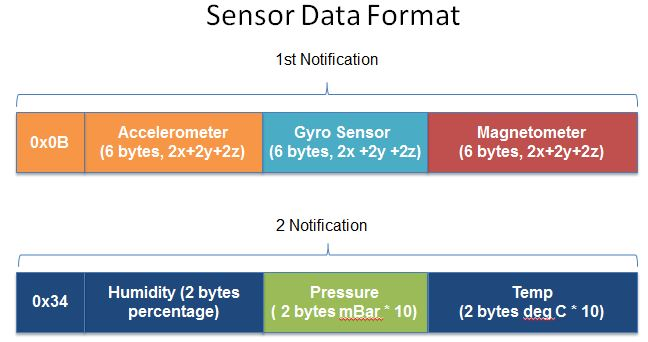
\includegraphics[scale=0.7]{PacketFormat.JPG}
	\end{figure}


\end{document}